\documentclass[a4paper,11pt]{article}
\usepackage[utf8x]{inputenc}
\usepackage[IL2]{fontenc}
\usepackage{times}
\usepackage{url}
\DeclareUrlCommand\url{\def\UrlLeft{<}\def\UrlRight{>} \urlstyle{tt}}
\usepackage[czech]{babel}
\usepackage[left=2cm,text={17cm, 24cm},top=3cm]{geometry}
\usepackage{amsmath}
\usepackage{graphics}
\usepackage{picture}
\usepackage[pdftex]{graphicx}
\usepackage{epstopdf}

\begin{document}
\begin{center}
  \Huge
  Dokumentace k~projektu IMS\\
  \Large
  Implementace knihovny pro generování pseudonáhodných čísel\\
  \large
  Autoři: Pavel Novotný (xnovot28), Ota Pavelek (xpavel08)

\end{center}
\section{Úvod}
Při simulacích [IMS, slide 8] se často používají náhodné jevy [IMS, slide 76] či procesy, neboť některé části modelů [IMS, slide 7] jsou neurčité nebo je neumíme popsat jinak. Jedná se například o popisy příchodů (např. zákazníků) v systémech hromadné obsluhy [IMS, slide 139], výskytu poruch[IMS, slide 94] nebo katastrof, určení doby obsluhy či doby životnosti nějakého zařízení. Především pro tvorbu simulačních modelů [IMS, slide 46] je tedy potřeba nástroj, který v průběhu simulace zajistí požadovanou náhodnost [IMS, slide 76] a to pokud možno rychle a přesně. Právě takovým nástrojem je zde dokumentovaná knihovna pro generování pseudonáhodných čísel [IMS, slide 100] nabízející tvůrci simulačního modelu na výběr z několika rozložení pravděpodobnosti [IMS, slide 90] výskytu žádané náhody.

Generátor pseudonáhodných čísel je program, jehož výstupem je deterministicky [IMS, slide 31] a efektivně určená posloupnost čísel taková, že je statisticky [IMS, slide 35] k nerozeznání od náhodné posloupnosti čísel \cite{wiki}. Cílem této knihovny je vytvořit implementaci generátoru pseudonáhodných čísel, takže bude snadno použitelná v simulačních modelech nebo jiných náhodnost požadujících programech.

\subsection{Zdroje faktů}
Problematika generování náhodnosti je poměrně dobře popsána a to jak samotné generování pseudonáhodných čísel v rovnoměrném rozložení [IMS, slide 92], tak také transformace [IMS, slide 105] z rovnoměrného rozložení do jiných žádaných rozložení.

Co se týče generování pseudonáhodných čísel, byly díky použitému generátoru s názvem Mersenne Twister [IMS, slide 104] hlavním zdrojem informací odborný článek \emph{Mersenne Twister: A 623-dimensionally equidistributed uniform pseudorandom number generator} \cite{Matsumoto} a osobní stránka jeho tvůrce, profesora Makoto Matsumota \cite{Matsumoto2}.

Transformace mezi pravděpodobnostními rozloženími si vyžádaly více faktických zdrojů, ovšem tím stěžejním byla kniha \emph{Numerical} Recipes \cite{NR}, která k tématu poskytla obsáhlé, ba až vyčerpávající informace. V některých případech bylo nahlédnuto do odborných vědeckých článků, na něž bude ve vhodnou dobu upozorněno.


\section{Rozbor tématu a použitých metod}
Jak už mohlo vyplynout z úvodu, dá se knihovna dekomponovat na dva dílčí podproblémy. Jedním z nich je generování pseudonáhodných čísel v rovnoměrném rozdělení pravděpodobnosti, druhým pak transformace rovnoměrného rozdělení pravděpodobnosti na jiná rozdělení. Zmíněnou dekompozici bude sledovat i struktura této kapitoly.

\subsection{Generování čísel v rovnoměrném rozdělení}
V teorii modelování [IMS, slide 8] na simulací se normalizované rovnoměrné rozdělení bere jako základ pro generování dalších rozdělení [IMS, slide 92]. Dobrá knihovna pro generování pseudonáhodných čísel by tedy měla implementovat zvláště dobře právě generátor pro toto rozdělení, protože na něm závisí i kvalita čísel vygenerovaných pomocí jiných rozdělení pravděpodobnosti. Přitom \emph{zvláště dobře} implementovaný (či navrhnutý) zde znamená rychlý, s co nejdelší periodou (počet čísel, po kterých se posloupnost začne opakovat) a se statisticky nezávisle generovanou posloupností [IMS, slide 104].

Algoritmů pro generování pseudonáhodných čísel v rovnoměrném rozdělení je celá řada, avšak ne všechny mají \emph{zvláště dobré} vlastnosti. V souvislosti se \emph{zvláště dobrými} algoritmy se v poslední dekádě mluví především o algoritmu Mersenne Twister [IMS, slide 104], známým též jako MT19937 \cite{Matsumoto}, který nejenže má velmi velkou periodu $2^{19937} – 1$, ale je také velmi rychlý a to i v porovnání s výpočetně jednoduchým lineárně kongruentním generátorem [IMS, slide 101] (oproti němu je však paměťově náročnější) \cite{Matsumoto}. Přes jistou nevýhodu, kterou je jeho nepoužitelnost pro kryptografické účely (pokud získáme posloupnost určité délky, můžeme odvodit zbytek) \cite{Matsumoto}, byl tento algoritmus vybrán, neboť knihovna najde své použití spíše při tvorbě simulačních modelů, kde zmíněný nedostatek nevadí.

Jako alternativa k algoritmu Mersenne Twister se nabízel algoritmus \emph{Complimentary-multiply-with-carry}, od výzkumníka na poli generátorů pseudonáhodných čísel George Marsaglii (též autor tzv. Diehard testů). Jeho algoritmus má větší periodu ($2^{131086}$), je rychlejší, ale paměťově náročnější \cite{jomasm}. Přestože byl vybrán Mersenne Twister (pro lepší dohledatelnost a větší známost), knihovnu lze jednoduše přizpůsobit i pro CMWC algoritmus, o čemž je pojednáno dále.

\subsection{Transformace rovnoměrného rozdělení na jiná rozdělení}
Rozdělení, která knihovna podporuje, jsou následující: rovnoměrné, exponenciální, normální, Weibullovo, Poissonovo a  gamma [IMS, slide 90]. Pro různá rozdělení byly použity různé metody transformace z výchozího rovnoměrného rozložení.

\subsubsection{Metoda inverzní transformace}
Inverzní transformace [IMS, slide 105] je způsob, jímž se dají náhodná čísla generovat přesně v daném rozdělení \cite{IMS2}. Metoda vychází z funkce inverzní k distribuční funkci požadovaného rozdělení, což však znemožňuje použitelnost této metody pro rozdělení, jejichž distribuční funkce [IMS, slide 82] buď nemají inverzní funkci nebo je tato inverzní funkce nevyjádřitelná elementárními funkcemi \cite{IMS2}.

V knihovně je metoda inverzní transformace použita pro rovnoměrné, exponenciální a Weibullovo rozdělení. Všechna rozdělení mají poměrně jednoduše vyjádřitelnou inverzní funkci k distribuční funkci. Podoba použitých inverzních funkcí daných rozdělení je uvedena dále.

\subsubsection{Metoda Ratio-of-Uniforms}
Pro některá rozdělení pravděpodobnosti existuje více způsobů transformace z rovnoměrného rozdělení, avšak ne všechny tyto způsoby jsou dostatečně efektivní. Kinderman a Monahan vytvořili kombinovanou transformační metodu, která je poměrně efektivní, přestože není implementačně složitá \cite{KM}. Metoda Ratio-of-Uniforms (česky snad „poměr rovnoměrných“) vychází z metody vylučovací [IMS, slide 105], ze které přebírá princip nacházení takových dvou náhodných rovnoměrně rozdělených čísel, že leží uvnitř specifického dvourozměrného tvaru. Z těchto dvou čísel je pak náhodné číslo cílového rozdělení vytvořeno výpočtem poměru původních dvou \cite{NR}. Důkaz platnosti metody je podán v \cite{KM} i \cite{NR}. Metoda byla použita pro generování náhodných čísel v normálním a v Poissonově rozdělení.

Co se týče normálního (Gaussova) rozdělení, byla použita implementace algoritmu, který vytvořil a v článku \emph{A Fast Normal Random Number Generator} publikoval Joseph L. Leva \cite{Leva}. Ten výpočetně optimalizoval metodu Ratio-of-Uniforms tak, že minimalizoval potřebný počet výpočtů logaritmu, přičemž nabízí i srovnání s dalšími algoritmy \cite{Leva}. Algoritmus od Leva je přesný a rychlý, takže při výběru metody nevzniklo žádné dilema. Alternativně by mohla být použita jedna z variant Box-Miller transformační metody.

Poissonovo rozdělení je jediné diskrétní rozdělení [IMS, slide 90] v dokumentované knihovně. Kniha \cite{NR} navrhuje a knihovna pro generování pseudonáhodných čísek implementuje dva způsoby generování čísel v Poissonově rozdělení, které se používají v závislosti na střední hodnotě rozdělení. První metodou je zmíněná Ratio-of-Uniforms s řadou výpočetních optimalizací, druhou pak metoda násobící (Multiplication Method) \cite{AD}, kterou jako první popsal Donald Knuth ve svém díle \emph{The Art of Computer Programming}, ale která je použitelná pouze pro nízké střední hodnoty $\lambda$ (pro ně je výpočet efektivní). Nutno zmínit, že v článku \cite{AD} je nabízena řada dalších alternativních metod pro výpočet včetně jejich srovnání, z něhož vyplývá, že Knuthova metoda je výhodná jen pro střední hodnoty nepřesahující hodnotu 5 \cite{AD}, tab. P]. Bohužel se zde nevyskytuje srovnání s metodou Ratio-of-Uniforms, avšak ta by dle \cite{NR} měla být rychlá i pro velmi velké střední hodnoty.

\subsubsection{Vylučovací metoda}
Vylepšená verze vylučovací metody [IMS, slide 105], jak ji navrhli Marsaglia a Tsang v \cite{Marsaglia} je použita pro generování gamma rozdělení. Základní princip metody spočívá ve vygenerování dvojice náhodných čísel v rovnoměrném rozdělení a testování zda vyhovují funkci hustoty cílového rozdělení [IMS, slide 105]. Pro gamma rozdělení je metoda upravena, přičemž více podrobností je uvedeno dále.

\section{Koncepce a analýza}

\subsection{Návrh programu}

Knihovna pro generování pseudonáhodných čísel využívá objektově orientovaný přístup ve svém návrhu (a posléze i v implementaci). Stanoveným cílem knihovny je dát uživateli možnost vytvořit jeden objekt, který umí generovat náhodnost všech rozdělení, a pokryje pro tyto účely potřeby daného lokálního prostoru, kde bude objekt moci až do svého zničení neustále poskytovat správná čísla. Uživateli však musí být umožněno vytvářet libovolný počet generátorů a to se stejnými i různými inicializačními hodnotami. Pokud bude uživatel knihovny chtít změnit základní generátor čísel v rovnoměrném rozdělení, musí být tato změna pro něj co nejméně náročná.

Ke splnění uvedených požadavků postačuje použití základních objektově orientovaných principů jako jednoduchá dědičnost a zapouzdření. Obrázek \ref{diagram1} zobrazuje, jak jednoduchá je struktura knihovny pro generování pseudonáhodných čísel. Dvě třídy ve vztahu rodič – potomek, kde rodič je libovolný generátor pseudonáhodných čísel v rovnoměrném rozdělení a potomek generátor rozdělení z něho transformovaných. Použitá dědičnost je jednoduchá, použitá k účelu snadné záměny rodiče bez nutnosti změn v potomku a všude využívá volání metod časnou vazbou.

\begin{table}[h]
\begin{center}
\scalebox{0.4}{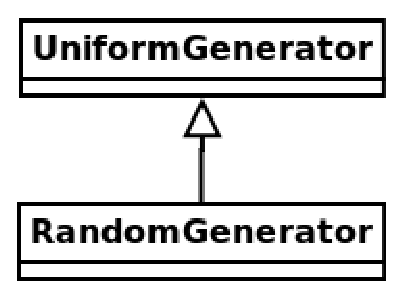
\includegraphics{Diagram1.eps}}
\caption{\label{diagram1}Struktura knihovny}
\end{center}
\end{table}
\subsection{Analýza rozdělení}

Nyní budou podrobněji rozebrána jednotlivá rozdělení pravděpodobnosti. Popis každého z nich zahrnuje informace obecného rázu, způsob značení, jak se může objevit v literatuře nebo v abstraktním modelu [IMS, slide 10] a příklady využití rozdělení v oblasti modelování a simulací. K tomu jsou uvedeny konkrétní postupy výpočtů tak, jak je implementuje knihovna. 

\subsubsection{Rovnoměrné rozdělení}
Rovnoměrné rozdělení [IMS, slide 92] je takové rozdělení, kdy náhodná veličina [IMS, slide 78] X nabývá se stejnou pravděpodobností, jakoukoliv hodnotu z intervalu $<a, b>$ \cite{INM}. Pokud jsou hodnoty $a = 0$ a $b = 1$, mluvíme o normované formě rovnoměrného rozdělení a takové rozdělení je základem pro generování dalších rozdělení [IMS, slide 92]. Rozdělení můžeme vyjádřit diskrétně i spojitě, avšak zde uvažujeme pouze vyjádření spojité.

Označení: R(a,b) nebo Uniform(a,b)

V modelování a simulacích je toto rozdělení důležité zejména z hlediska generování náhodných čísel, která jsou dále transformována na jiná rozložení. Při modelování se použije například pro doby čekání nebo doby různých činností.

Rovnoměrné rozdělení poskytuje knihovna jako výchozí rozdělení, avšak v normalizované podobě. Pro zobecněnou formu je potřeba použít nějakou transformační metodu, jíž se nabízí metoda inverzní transformace. Distribuční funkce rovnoměrného rozdělení v intervalu $<a, b>$ [IMS, slide 92] je $$F(x) = \frac{(x-a)}{(b-a)}$$ Vyjdeme-li ze vztahu $$u = F(x), u \in Uniform(0, 1)$$pak $$u = \frac{(x-a)}{(b-a)}$$ a po jednoduché úpravě dostaneme 
\begin{eqnarray}\label{inverzniUniform}
x = a + u * (b-a)
\end{eqnarray}
což je výsledná inverzní funkce $$x=F^{-1}(u)$$ Jinými slovy máme-li náhodné číslo u náležící do intervalu $<0, 1>$, potom funkce \ref{inverzniUniform} jej převede na náhodné číslo x z intervalu $<a, b>$.

\subsubsection{Normální rozdělení}

Normální (též Gaussovo) rozdělení je nejdůležitějším spojitým rozdělením \cite{INM}, slide 60]. Využívá se ve statistice (chyby měření) a při aproximaci mnoha jiných, spojitých i diskrétních, rozdělení. Množství náhodných veličin v různých odvětvích vědy a techniky má normální rozdělení. Graf hustoty pravděpodobnosti tohoto rozdělení nese vlastní název Gaussova křivka; ta je specifická tím, že je souměrná podle osy $x \equiv \mu$ a v bodě $x = \mu$ má maximum.

Jeho parametry jsou též jeho charakteristikami, přičemž střední hodnota $$E(X) = \mu$$ a rozptyl $$D(X) = \sigma^2$$Podobně jako u rovnoměrného rozdělení, pokud parametry nabývají hodnot $\mu = 0$ a $\sigma=1$, mluvíme o normované (též standardizované) formě normálního rozdělení. \cite{INM}

Označení: $N(\mu, \sigma)$

Existuje velká řada jevů (např. jevy s vlivem většího počtu nezávislých faktorů [IMS, slide 96]), které odpovídají normálnímu rozdělení, takže se v simulacích jedná o poměrně častě využívané rozdělení. Také se může vyskytnout při použití metody Monte Carlo [IMS, slide 114] nebo při vyhodnocování výsledků simulací.

Pro výpočet normálního rozdělení je v knihovně použita transformační metoda Ratio-of-Uniforms, jejíž princip byl nastíněn v přecházející kapitole. Několikastránkový popis celého algoritmu je napsán v článku \cite{Leva}, kam odkazujeme zájemce o něj.

\subsubsection{Exponenciální rozdělení}

Exponenciální rozdělení je spojité rozdělení modelující situace, kdy opakovaně a nezávisle dochází k výskytu náhodné události a zároveň nenastane více těchto situací najednou \cite{INM}. Rozdělení má vhodné vlastnosti pro upotřebení v teorii spolehlivosti \cite{IASTAT}.

Střední hodnota $$E(X) = \frac{1}{\lambda}$$ rozptyl $$D(X) = =\frac{1}{\lambda^2}$$

Označení: $E(\lambda)$ nebo $Exp(\lambda)$ \cite{INM}.

Jedná se o velmi významné rozdělení pro modelování a simulace. V systémech hromadné obsluhy je  obvykle využité pro doby mezi příchody do front či pro doby čekání ve frontách. Používá se pro modelování doby čekání na výskyt nějakého jevu, takže dobře popisuje například dobu života zařízení, u kterého dochází k poruše ze zcela náhodných příčin (nikoliv z důsledků opotřebení) \cite{IASTAT}.

Protože existuje inverzní funkce k distribuční funkci exponenciálního rozdělení a je vyjádřitelná pomocí elementárních matematických funkcí, můžeme ji použít pro transformaci z rovnoměrného rozdělení. Distribuční funkce je 

$$
{F(x)} = \left\{
\begin{array}{ll}
 1 - e ^{-\lambda x} & \quad\text{pro } x \geq 0  \\
 0 & \quad\text{pro } x < 0
\end{array}
\right.
$$

Řekněme, že $u \in Uniform(0,1)$ a $u = F(x)$. Potom po úpravě 
$$-\lambda x = ln(1-u)$$
$$x = -\frac {ln(1-u)}{\lambda}$$
Můžeme však ušetřit jedno odečítání, protože $$(1-u) \in Uniform(0,1)$$ stejně jako $$u \in Uniform(0,1)$$ takže výsledná funkce transformující normalizované rovnoměrné rozdělení na exponenciální je 
$$x = -\frac{ln(u)}{\lambda}$$

POZN.: Knihovna pro generování pseudonáhodných čísel i tento dokument používá jako parametr exponenciálního rozdělení hodnotu $\lambda$, avšak někdy se exponenciální rozdělení definuje parametrem $\delta = \frac{1}{\lambda}$, tedy svou střední hodnotou.

\subsubsection{Weibullovo rozdělení}

Weibullovo rozdělení popisuje takovou náhodnou veličinu X, která vyjadřuje čekání na událost, jež se může může dostavit s šancí úměrnou mocninné funkci dosud pročekané doby [INM, slide 58]. Používá se všude tam, kde nevyhovuje „rozdělení bez paměti“, tedy exponenciální \cite{IASTAT} \cite{HOMEN}. V praxi se jedná o zařízení, kde se projevuje mechanické opotřebení nebo únava materiálu \cite{HOMEN}. Toto spojité rozložení má dva kladné parametry, které se nazývají měřítko a tvar (forma) \cite{Toupal} \cite{INM}. Pokud je tvar $>$ 1, je charakterizováno zařízení, u kterého se pravděpodobnost poruchy zvyšuje, naopak pro tvar $<$ 1 se pravděpodobnost poruchy snižuje. Je-li tvar = 1, jedná se o exponenciální rozdělení \cite{Toupal}.

Označení: W(tvar, měřítko), Wb(tvar, měřítko) nebo Weibull(tvar, měřítko).

Při modelování spolehlivosti či selhání například výrobního zařízení se uplatní Weibullovo rozdělení před exponenciálním. Díky simulacím pak lze usnadnit rozhodování, zda se má modelované zařízení nahradit dříve než selže. Dle \cite{Toupal} se využívá i k prezentování výrobních a dodacích časů v průmyslu nebo k předpovědím počasí.

Distribuční funkce Weibullova a exponenciálního rozdělení si jsou dost podobné, neboť Weibullovo rozdělení je (jistým způsobem) zobecněné exponenciální rozdělení \cite{NR}. Podobné je i odvození inverzní funkce k distribuční funkci, která je definována jako $$F(x) = 1 – e^{-(\frac{x}{\beta})^{\alpha}},$$ kde $\beta$ je měřítko a $\alpha$ je tvar. 

Řekněme, že $u \in Uniform(0,1)$ a $u = F(x)$, takže po úpravách získáme nejprve 
$$\left(\frac{x}{\beta}\right)^\alpha = -ln(1-u)$$ 
a poté 
$$x = beta * [-ln(1-u)]^{\frac{1}{\alpha}}.$$ 
Podobně jako bylo odstraněno odčítání v argumentu logaritmu u exponenciálního rozdělení, jde odstranit i zde.

\subsubsection{Gamma rozdělení}

Spojité rozdělení, které podobně jako rozdělení Weibullovo má dva parametry pojmenované tvar a měřítko. Odpovídá době čekání na n-tou událost, kde n je parametr tvar. Pro celočíselný tvar přechází na Erlangovo rozdělení \cite{Wiki2}, pro tvar = 1 se stává exponenciálním rozdělením \cite{Wgamma}. V kombinaci s Poissonovým rozdělením tvoří negativní binomické rozdělení. Využití tohoto rozdělení najdeme (kromě modelování a simulací) ve statistice a meteorologii. \cite{Wiki2}

Označení: Gamma(k, $\Pi)$ nebo $\Gamma(k,  \Pi)$.

Využití v simulacích je možné pro modely života (umírání) \cite{Wgamma} \cite{Wiki2} nebo také tam, kde nachází uplatnění Erlangovo rozdělení, tedy modelování příchodů, dob čekání nebo u compartment models (česky snad „členěné modely“).

V \cite{NR} jsou uvedené dvě metody transformace a to pro pro různé hodnoty parametru k (tvar). Pro $k < 1$ je využito vztahu $$y*u^{\frac{1}{k}} \equiv \Gamma(k, 1), \text{kde } y \equiv \Gamma(k+1, 1) \text{ a } u \equiv Uniform(0, 1) \text{\cite{NR}}.$$ Pro $k > 1$ je použita upravená verze vylučovací metody, kterou vytvořili Marsaglia a Tsang a která využívá Gaussovu křivku, takže její rychlost závisí na rychlosti počítání nejen rovnoměrného ale i normálního rozdělení. Jelikož je metoda poměrně složitá a její výklad by zabral několikero stran, uvádíme pouze informační zdroj, jímž je \cite{Marsaglia}. 

\subsubsection{Poissonovo rozdělení}

Poissonovo rozdělení je jediné diskrétní rozdělení v knihovně pro generování pseudonáhodných čísel. Úzce souvisí s exponenciálním rozdělením, které popisuje dobu mezi dvěma událostmi, zatímco Poissonovo počet výskytů události za určitou dobu \cite{INM}. Použijeme-li parametr rozdělení $\lambda$, který zároveň představuje střední hodnotu i rozptyl, můžeme tvrdit, že k výskytu události dochází průměrně jednou za $\frac{1}{\lambda}$ časových jednotek, tj. $\lambda$-krát za jednu časovou jednotku \cite{INM}. Pomocí Poissonova rozdělení jde za určitých podmínek aproximovat binomické rozdělení \cite{INM} a existuje také vztah pro převod na rozdělení exponenciální.

Označení: P($\lambda$) nebo Poisson($\lambda$)

Poissonovo rozdělení je pro modelování a simulace důležité podobně jako jeho exponenciální protějšek. Modeluje se s ním počet příchodů za jednotku času v systémech hromadné obsluhy nebo obecně počty jakýchkoliv jevů vyskytujících se v určitém časovém kvantu [IMS, slide 91]. 

Stejně jako u normálního rozdělení je pro transformaci z rovnoměrného do Poissonova rozdělení použita metoda Ratio-of-Uniforms, která je tedy evidentně použitelná i pro diskrétní rozdělení. Trik převodu reálných hodnot, které jsou umístěné uvnitř metodou žádaného planárního útvaru, na hodnoty diskrétní spočívá v jednoduchém ořezání desetinné části \cite{NR}. Pro další detaily však musí zájemce prostudovat principy metody Ratio-of-Uniforms v knize \cite{NR}, protože zde není dostatek prostoru tuto metodu vysvětlovat.

\section{Architektura knihovny}

Jak již bylo řečeno návrh knihovny využívá objektově orientované paradigma, které se přirozeně promítne také do implementace, pro níž byl vybrán jazyk C++, který toto paradigma podporuje. C++ je rychlý kompilovaný přenositelný jazyk, jenž navíc nabízí techniky generického programování, neboli v terminologii jazyka šablony. Struktura dědičnosti tříd tak, jak byla definována v návrhu je v implementaci rozšířena o čistě virtuální třídu \emph{AbstractUniformGenerator}, která definuje rozhraní pro základní generátor náhodných čísel v rovnoměrném rozdělení, řekněme třeba \emph{UniformGenerator}. Jeho potomkem je pak šablona třídy \emph{RandomGenerator}, jejímž parametrem je právě onen generátor náhodnosti s rovnoměrným rozdělením, což uživateli umožňuje změnu základního generátoru při vytváření instance třídy \emph{RandomGenerator} za jakýkoliv jiný generátor bez nutnosti zasahovat do kódu knihovny. Jedinou podmínkou je, že uživatelův \emph{UniformGenerator} bude mít stejný protokol jako \emph{AbstractUniformGenerator} tedy jinak řečeno, bude jeho potomkem.

Knihovna nabízí pouze jeden generátor pseudonáhodných čísel s rovnoměrným rozdělením, jenž implementuje algoritmus Mersenne Twister. Jedná se o převzatou původní implementaci, kterou v jazyce C vytvořili a pod volnou licencí v \cite{Matsumoto} publikovali Matsumoto a Nishimura a kterou do jazyka C++ portoval Jasper Bedaux. V kódu bylo sice provedeno několik změn, ale jedná se spíše o změny formálního rázu za účelem přizpůsobení návrhu knihovny. Základní vlastnosti a srovnání algoritmu se v tomto dokumentu již objevily a jeho podrobný popis je podán tvůrci v článku \cite{Matsumoto}.

Transformace z rovnoměrného rozdělení do všech šesti rozdělení pravděpodobnosti, která knihovna podporuje, jsou implementovány v šabloně třídy \emph{RandomGenerator} jako její veřejné metody. Použité algoritmy jsou jak původní tak i převzaté a již byly detailněji rozebrány v přecházející části tohoto dokumentu, kde jsou uvedeny postupy odvození (je-li použita metoda inverzní transformace) nebo alespoň zdroje z nichž byly algoritmy čerpány. Z hlediska implementace však jistě stojí za zmínku mechanizmus uložení některých výsledků mezivýpočtů, který je použit pro urychlení generování Poissonova rozdělení za předpokladu, že je aspoň dvakrát za sebou použit stejný parametr. Jinými slovy, je zefektivněno časté po sobě jdoucí generování Poissonova rozdělení. 

Implementace knihovny je kompletně celá umístěna v hlavičkových souborech a to jednak, protože je to nutnou podmínkou při použití šablon, a jednak z pragmatických důvodů proto, aby se uživatel nemusel starat o kompilaci knihovny a mohl ji jednoduše přiložit direktivou include. Ke knihovně je přiložena implementace funkce logaritmus gamma funkce, jež je použita v některých algoritmech pro urychlení výpočtu faktoriálu \cite{NR}. Tato funkce je sice součástí chystaného standardu C++0x jazyka C++, který je na některých platformách již nyní k dispozici ve standardní knihovně funkcí (ač má být oficiálně vydán na až jaře roku 2011) avšak zatím by bez ní knihovna nebyla úplná. V budoucnu, až se standard C++0x rozšíří, jí bude možno z knihovny odstranit.

\section{Testování}
Pro testování byly použity platformy Unix a MS Windows. Otestované kompilátory jsou následující:
\begin{itemize}
\item gcc version 4.4.3, 64-bitové PC
\item gcc version 4.4.4, 32-bitové PC
\item MingW-32
\end{itemize}

Knihovna je bez problémů přenositelná. Kromě standardní knihovny funkcí nejsou použity žádné jiné knihovny ani moduly jazyka.

\subsection{Testování správnosti generovaných rozdělení}

Důležitým milníkem ve vývoji knihovny bylo otestování správnosti generování implementovaných pravděpodobnostních rozdělení, respektive správnosti transformačních metod. Výstupem testovacího programu je posloupnost čísel v určitém pravděpodobnostním rozdělení a tu je potřeba ověřit.

Existuje sice řada testů, které matematicky dokáží zda daná posloupnost čísel náleží určitému rozdělení pravděpodobnosti, pro testování knihovny byl však vybrán méně exaktní test. Byly vytvořeny skripty pro program gnuplot, což je program určený pro počítačové kreslení grafů, které do jednoho svého výstupu, jímž je rastrový obrázek, vykreslí jeden histogram náhodné posloupnosti 100 000 hodnot a k tomu odpovídající analytické vyjádření funkce hustoty pravděpodobnosti daného rozdělení. Každé rozdělení je takto testováno několikrát, vždy s jinými parametry. Histogram posloupnosti a křivka funkce hustoty pravděpodobnosti spolu musí vždy přesně korelovat. U některých rozdělení odhalila testovací metoda v průběhu testování chyby, které, jak se později ukázalo, byly implementačního rázu; například opačné znaménko u výpočtu v algoritmu transformační metody normálního rozdělení. Chyba se projevila tak, že histogram vykazoval výchylky (ne na celém svém rozsahu) od analytického vyjádření hustoty pravděpodobnosti.

Všechna rozdělení úspěšně prošla řadou testů s různými parametry. 

Ke knihovně jsou přiloženy také testovací skripty pro program gnuplot, které se spouští pomocí testovacího programu (je třeba mít nainstalovaný program gnuplot), takže je možno vyzkoušet a nahlédnout na výsledky tří vybraných posloupností pro každé rozložení (každá posloupnost má samozřejmě jiné přednastavené parametry).

Pozn.: Grafický výstup nebude fungovat na platformě MS Windows.

\section{Závěr}
Byla vytvořena knihovna pro generování pseudonáhodných čísel implementující šest pravděpodobnostních rozdělení pro potřeby modelování a simulací, která jsou generována transformací z volitelného generátoru rovnoměrně rozložené náhodnosti. Knihovna se uplatní při psaní simulačních modelů v jazyce C++, jejichž cílem je efektivní a přesná simulace. Použití knihovny je tak jednoduché jako vložení hlavičkového souboru a vytvoření instance třídy, přičemž má uživatel možnost použít vlastní generátor rovnoměrného rozdělení, pokud nechce použít výchozí, byť kvalitní.

Návrh a architektura knihovny včetně popisu použitých metod a postupů jsou zdokumentovány, aby pomohly pochopit, jakým způsobem knihovna pracuje, jak může být použita či případně upravena. Dokumentace knihovny si nekladla za cíl dopodrobna vyložit všechny detaily a vysvětlit všechny algoritmy. Mnoho věcí zůstalo skryto, ale vždy bylo ukázáno, kde je možno je najít. To nejdůležitější, jímž je nastínění celkové problematiky, kterou tvorba knihovny pro generování pseudonáhodných čísel představuje, je v dokumentaci obsaženo.

\newpage
\renewcommand{\refname}{Bibliografie}
\bibliographystyle {czechiso}
\bibliography {zdroje}
\end{document}
